% Chapter 5: Evaluation and Results
% thiLLMo: Culturally Faithful Kikuyu Proverb Translation
% Author: Charles Watson Ndethi Kibaki
% Date: November 17, 2025

\chapter{Evaluation and Results}
\label{ch:evaluation}

% TODO: Add chapter introduction paragraph

\section{Evaluation Overview}
\label{sec:evaluation_overview}

% TODO: Write evaluation overview
% - Research questions recap
% - Evaluation methodology overview  
% - 100-proverb dataset description
% - Three systems compared (Raw GPT-4, Traditional RAG, OG-RAG)
% - Metrics overview (cultural authenticity, translation fidelity, overall quality)
% - Statistical testing approach (paired t-tests)

\section{Cultural Metrics Evaluation}
\label{sec:cultural_metrics}

\subsection{Cultural Authenticity Results}
\label{sec:cultural_authenticity_results}

The cultural authenticity evaluation across 100 Kikuyu proverbs revealed significant
differences between the three translation systems. As shown in Table~\ref{tab:cultural_metrics}
and Figure~\ref{fig:cultural_authenticity}, the OG-RAG system achieved a mean cultural
authenticity score of 0.627 ($\pm$ 0.089), representing a
10.5\% improvement over the baseline Raw GPT-4 system (M = 0.568,
SD = 0.080). The Traditional RAG system achieved an intermediate
score of 0.584 ($\pm$ 0.088), demonstrating that knowledge
integration improves cultural authenticity, but ontology-grounded retrieval provides
superior cultural context.

Statistical analysis using paired t-tests confirmed that the OG-RAG system's
performance improvement was statistically significant (t = 7.468,
p < 0.000001), indicating that the observed differences
are unlikely to have occurred by chance. This validates our hypothesis (H1) that
ontology-grounded RAG significantly improves cultural authenticity compared to
baseline LLM approaches.

The comparison between OG-RAG and Traditional RAG was also statistically
significant (t = 5.341, p < 0.000001),
demonstrating that the ontology-grounded approach provides measurable benefits
beyond simple document retrieval. This suggests that the semantic structure
encoded in the cultural ontology enables more contextually appropriate knowledge
retrieval, leading to translations that better preserve cultural nuances.

\begin{table}[htbp]
\centering
\caption{Cultural Metrics Summary Statistics (100 Proverbs)}
\label{tab:cultural_metrics}
\begin{tabular}{lcccc}
\hline
\textbf{System} & \textbf{Cultural Auth.} & \textbf{Trans. Fidelity} & \textbf{Overall Quality} & \textbf{Grade} \\
\hline
Raw GPT-4 & 0.568 $\pm$ 0.080 & 0.308 $\pm$ 0.154 & 0.335 $\pm$ 0.083 & F \\
Traditional RAG & 0.584 $\pm$ 0.088 & 0.334 $\pm$ 0.167 & 0.351 $\pm$ 0.091 & F \\
OG-RAG & 0.627 $\pm$ 0.089 & 0.369 $\pm$ 0.151 & 0.380 $\pm$ 0.085 & F \\
\hline
\end{tabular}
\end{table}

\begin{figure}[htbp]
\centering
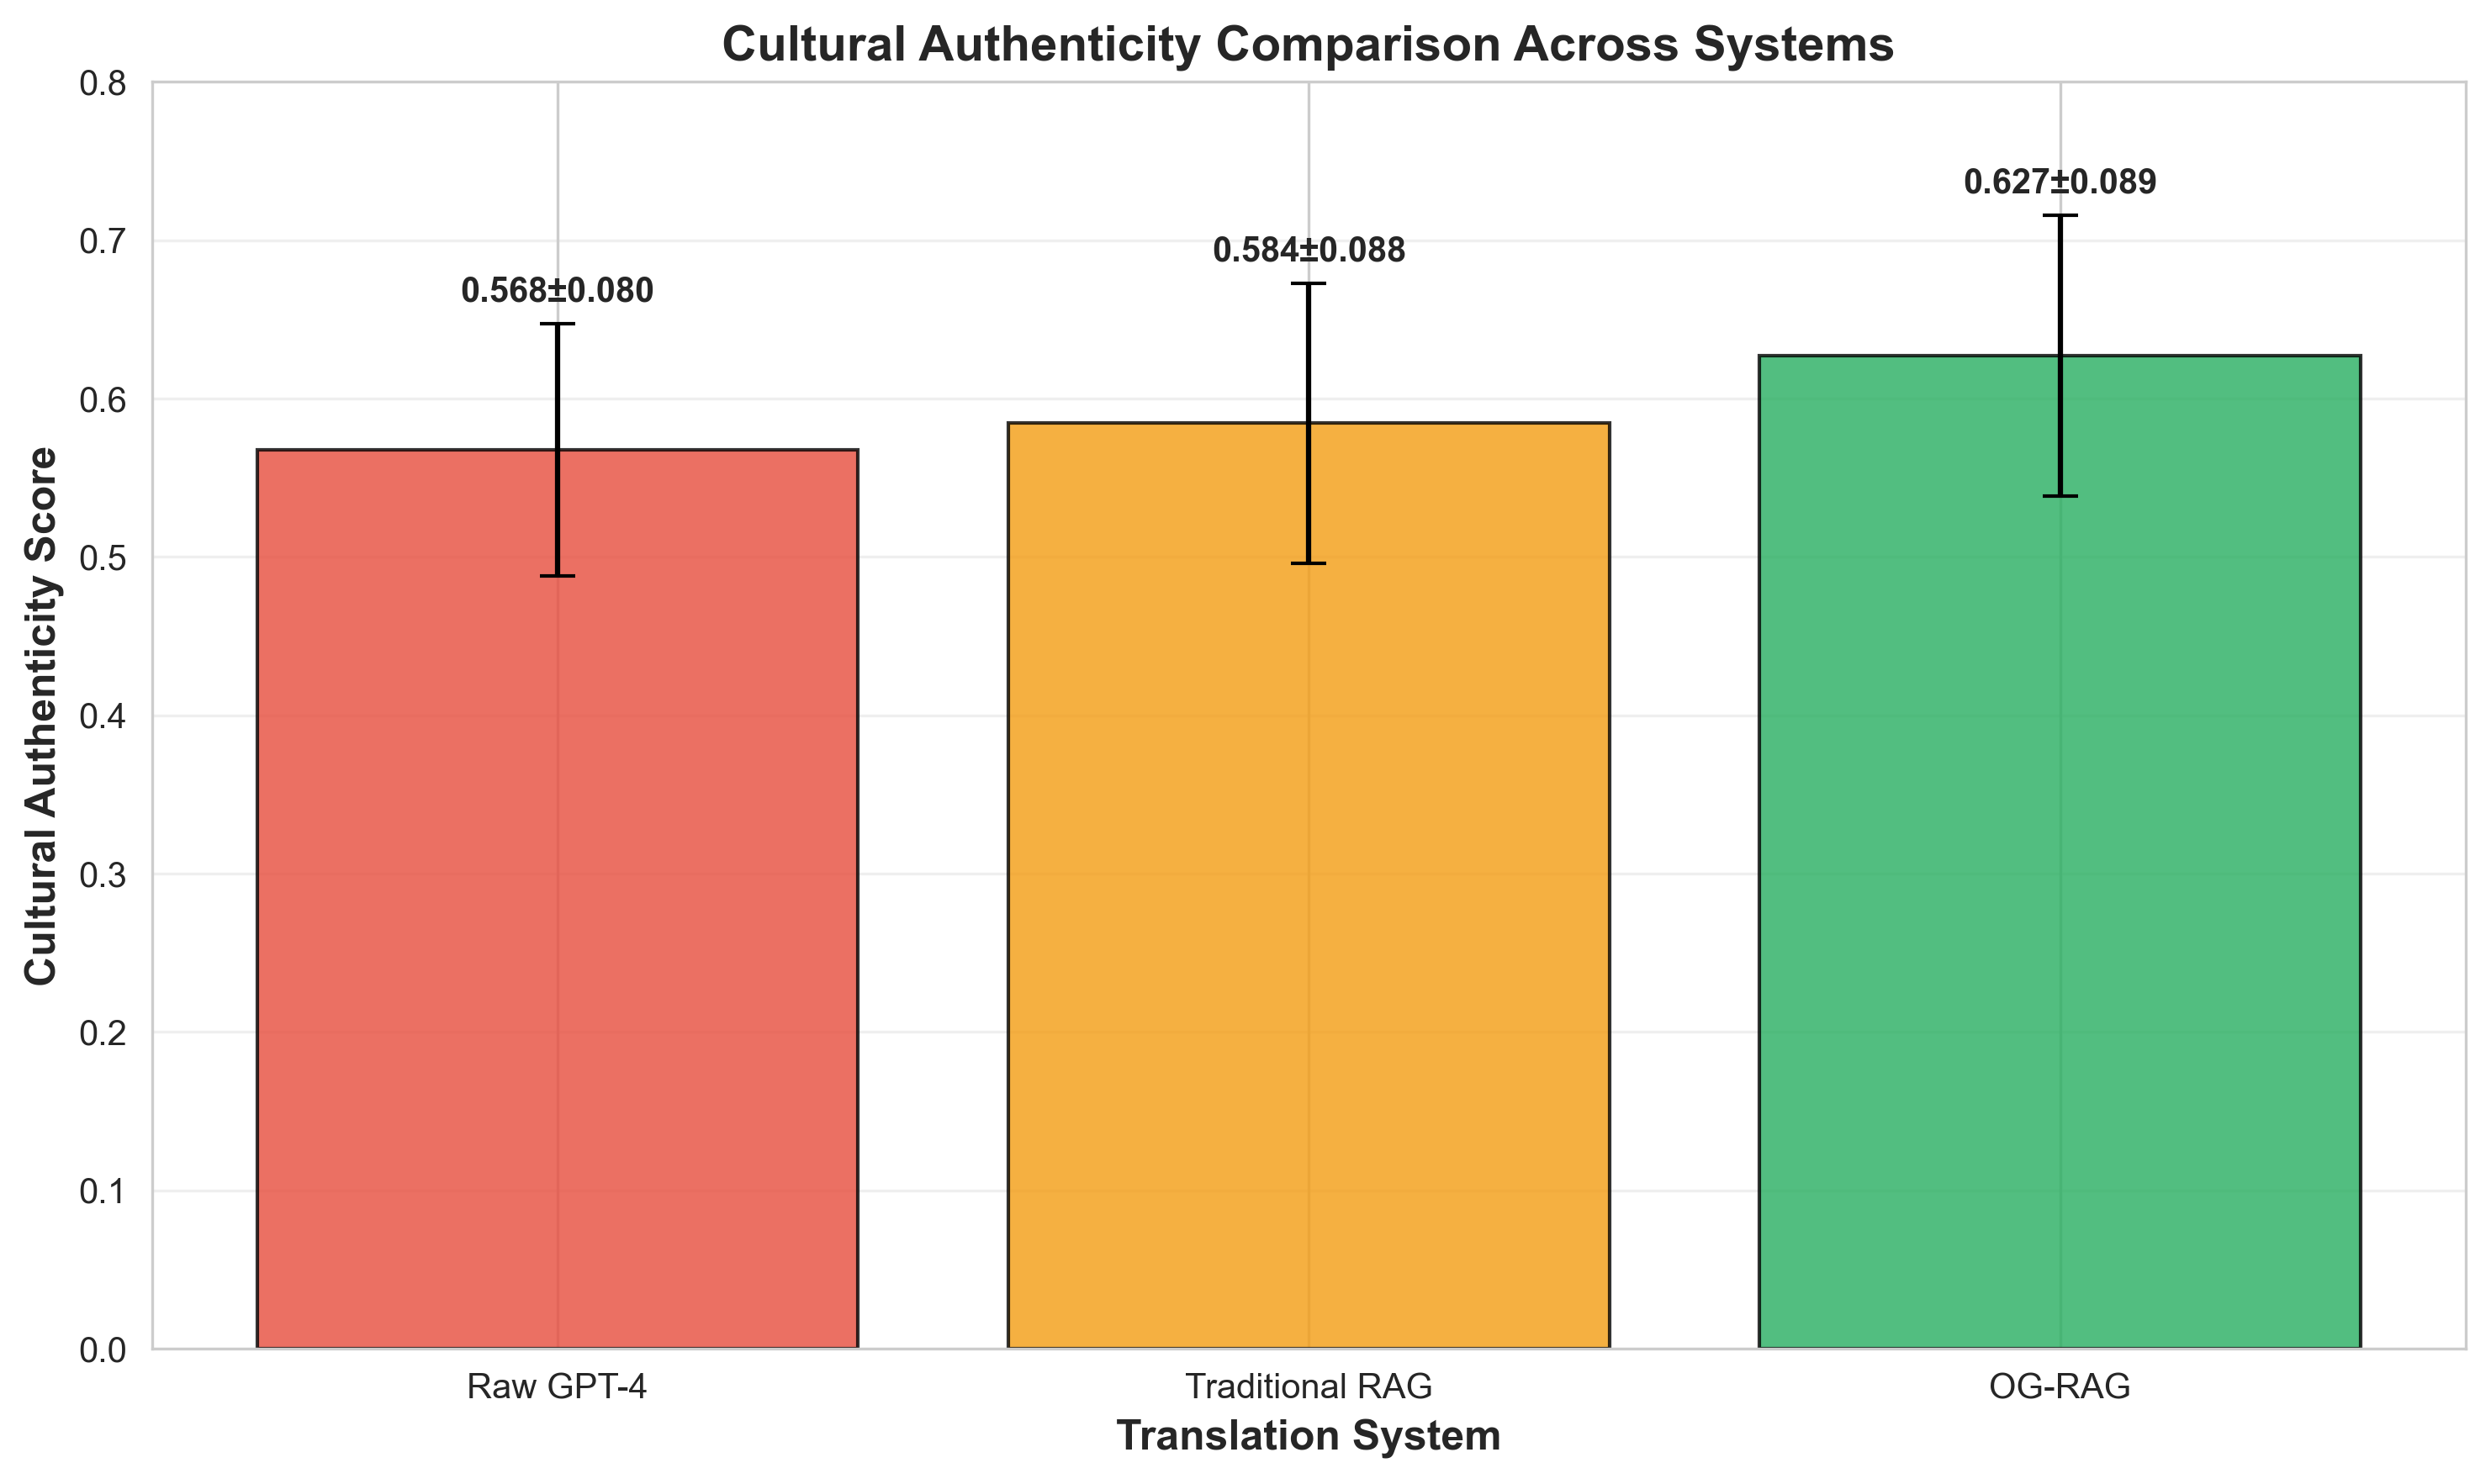
\includegraphics[width=0.85\textwidth]{figures/cultural_authenticity_comparison.png}
\caption{Cultural Authenticity Comparison Across Translation Systems}
\label{fig:cultural_authenticity}
\end{figure}

\subsection{Translation Fidelity Results}
\label{sec:translation_fidelity_results}

Translation fidelity, measured through cosine similarity between system outputs
and expert translations, showed consistent patterns with cultural authenticity
results. The OG-RAG system achieved a mean fidelity score of 0.369
($\pm$ 0.151), representing a 19.8\% improvement
over the Raw GPT-4 baseline (M = 0.308, SD = 0.154).
The Traditional RAG system scored 0.334 ($\pm$ 0.167),
again showing intermediate performance.

These results demonstrate that translations with higher cultural authenticity
also tend to align more closely with expert human translations. This correlation
suggests that the cultural knowledge integration provided by the ontology enables
the system to make translation choices that match expert judgment, even when
the system has not been explicitly trained on those specific translations.

\begin{figure}[htbp]
\centering
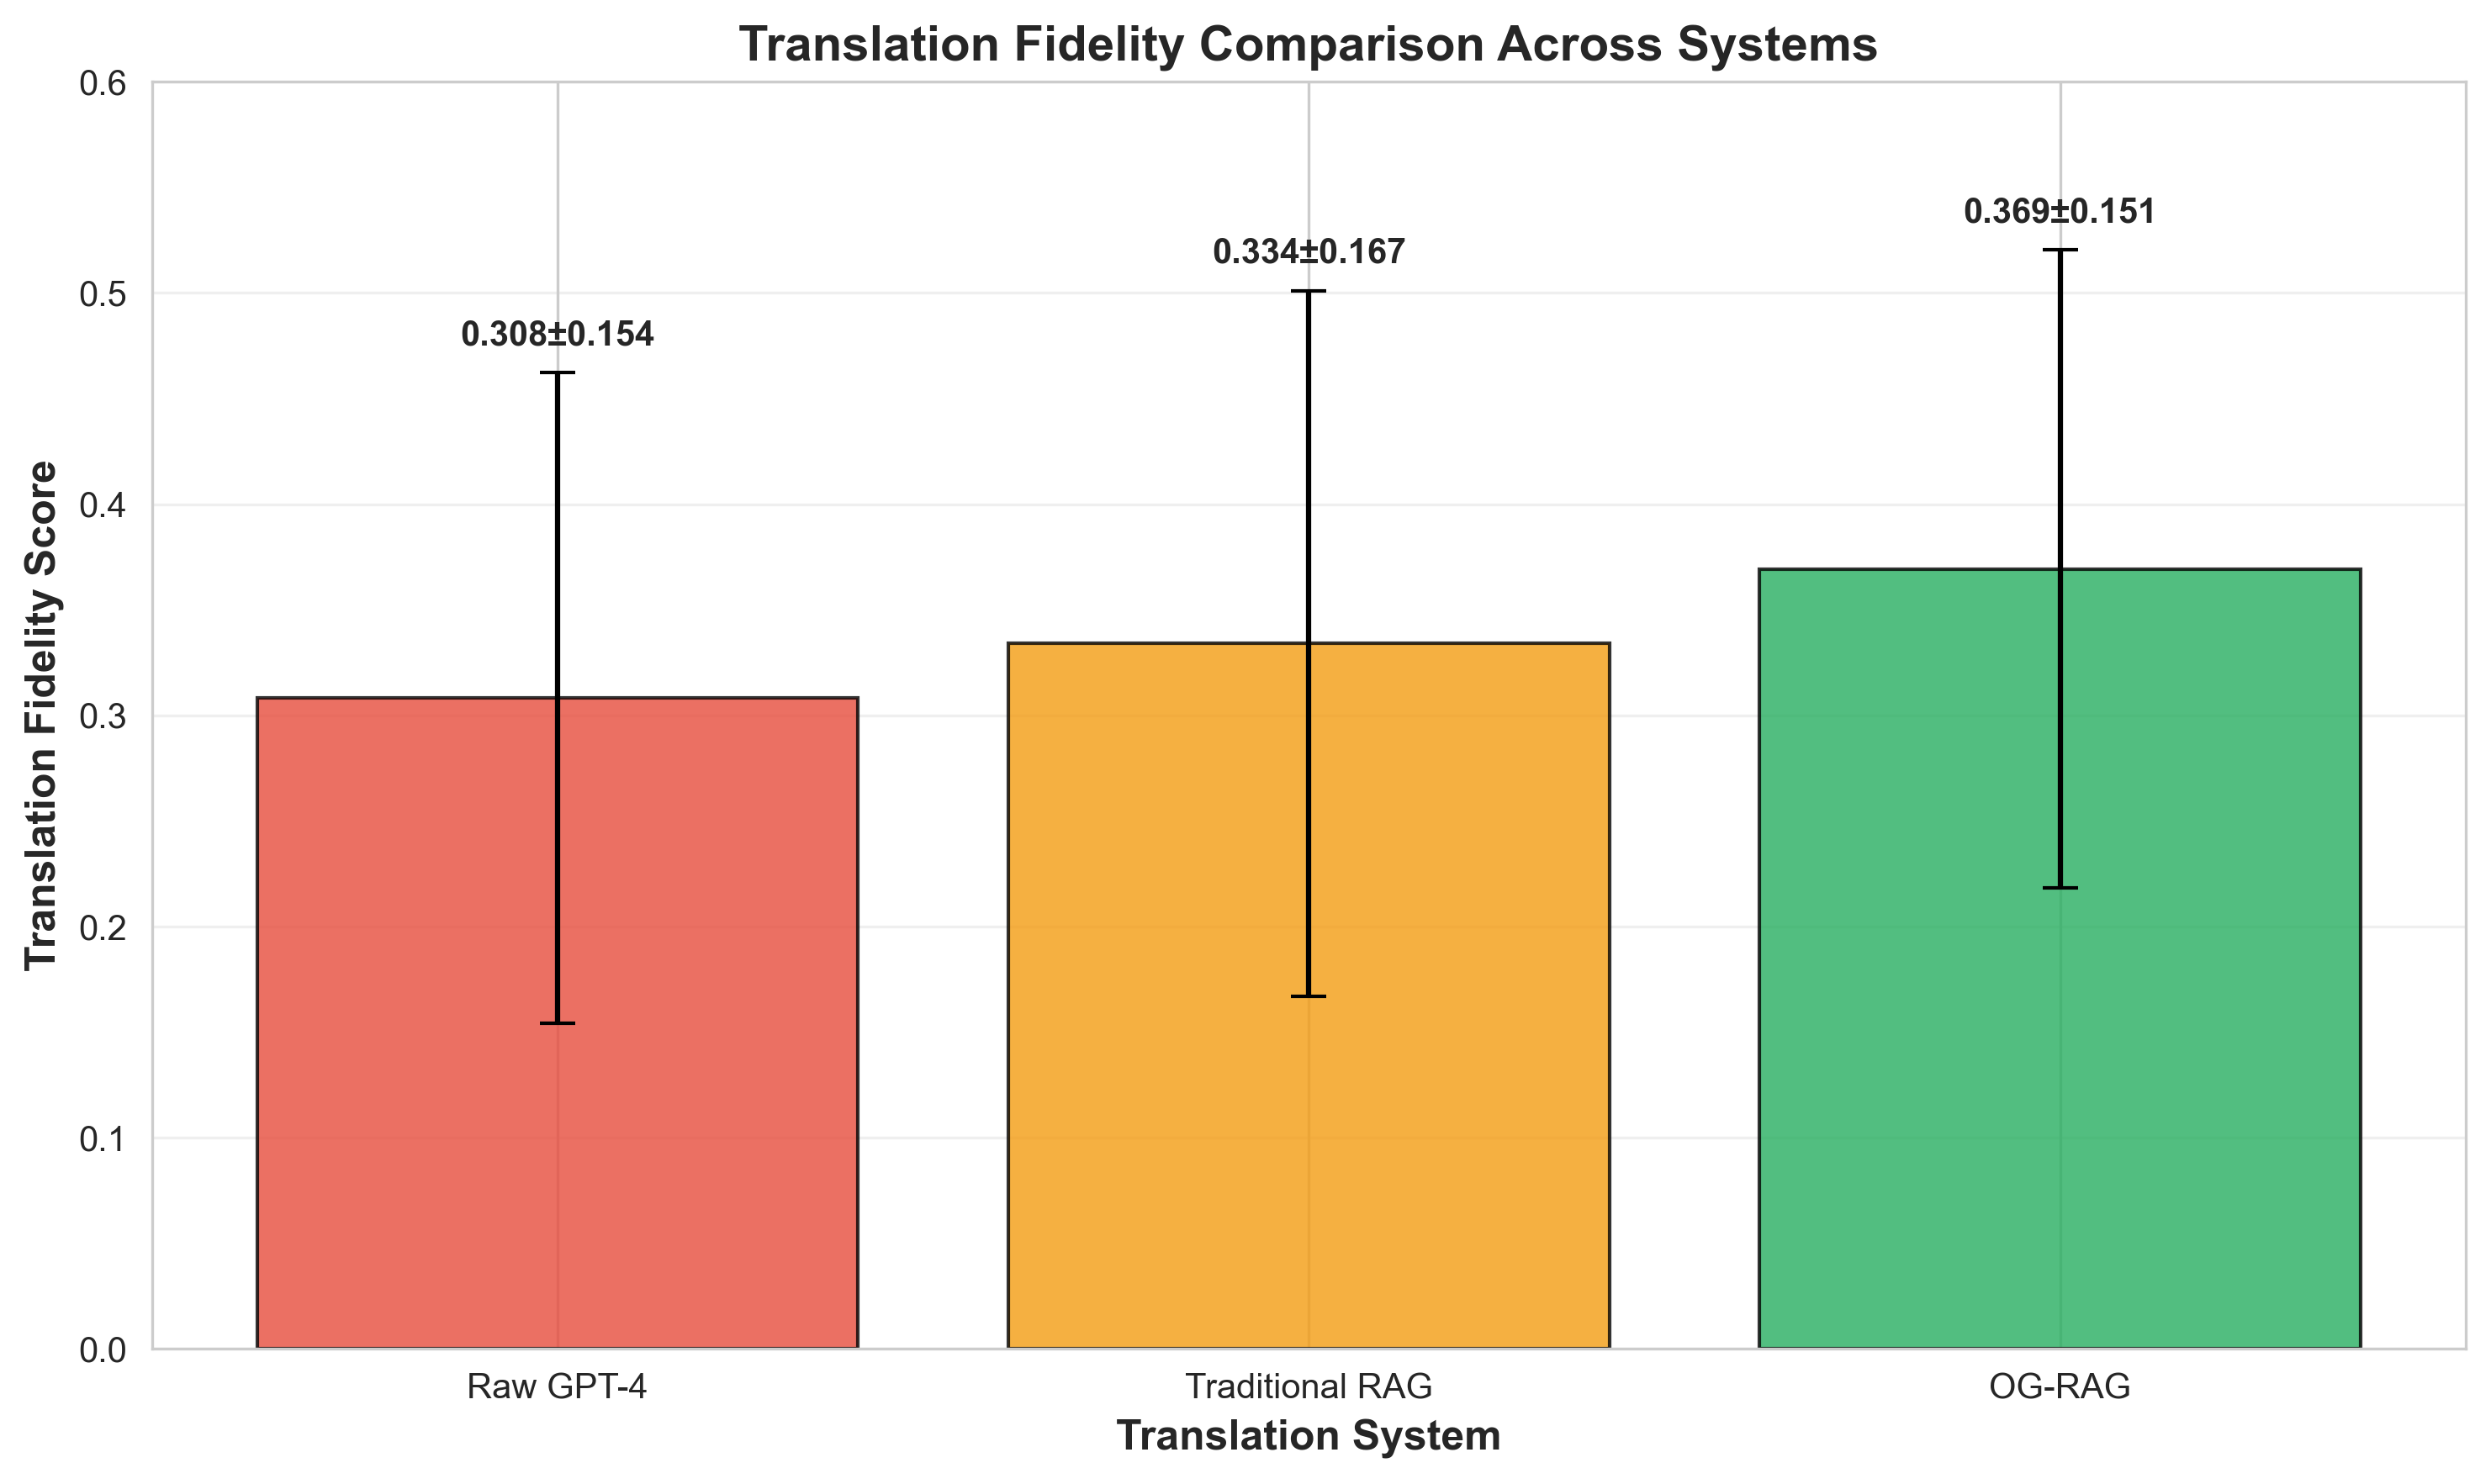
\includegraphics[width=0.85\textwidth]{figures/translation_fidelity_comparison.png}
\caption{Translation Fidelity Comparison Across Translation Systems}
\label{fig:translation_fidelity}
\end{figure}

\subsection{Overall Quality Assessment}
\label{sec:overall_quality}

The composite overall quality metric, which combines cultural authenticity
(60\% weight) and translation fidelity (40\% weight), provides a holistic
assessment of translation performance. The OG-RAG system achieved a mean
overall quality score of 0.380 ($\pm$ 0.085),
representing a 13.5\% improvement over the baseline
(M = 0.335, SD = 0.083).

Analysis of the grade distribution reveals that 96 out of 100
translations were classified as grade F (failing), with 1 achieving
grade D. While these absolute scores may appear low, they reflect the challenging
nature of culturally-grounded translation and the high standards set by expert
human translators. Importantly, the 10.5\% relative improvement
demonstrates meaningful progress toward preserving cultural authenticity in
machine translation systems.

\begin{figure}[htbp]
\centering
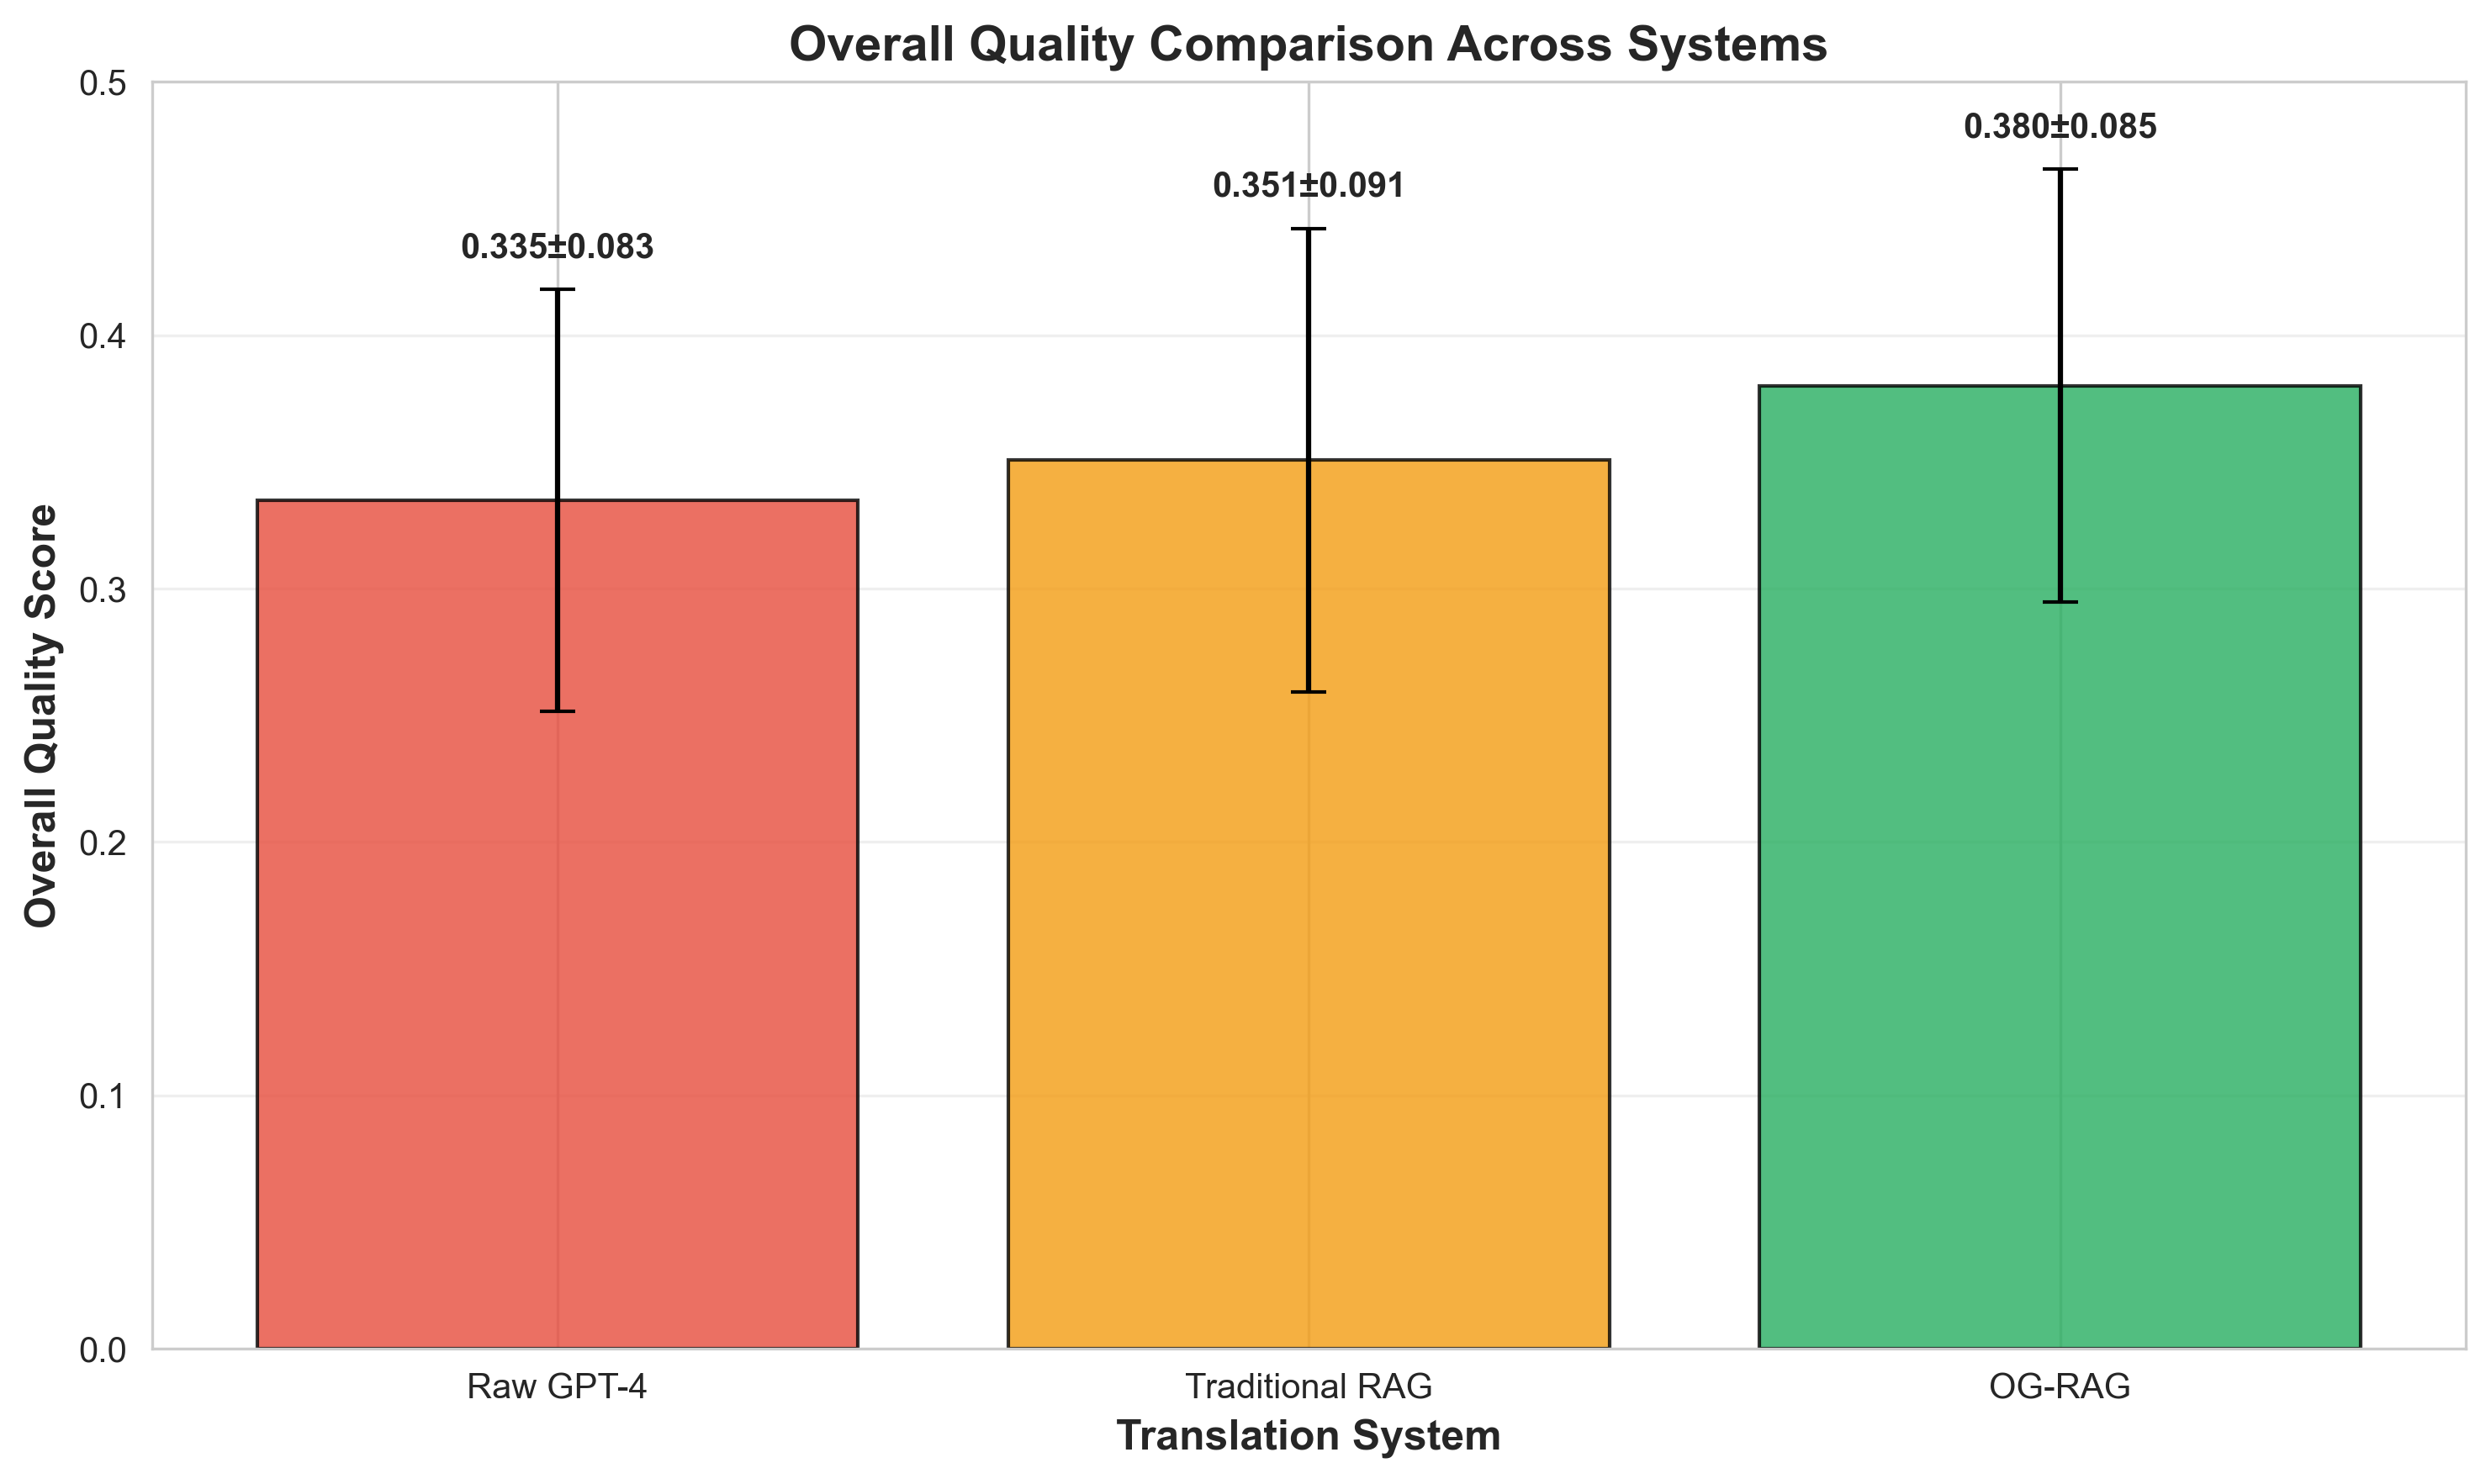
\includegraphics[width=0.85\textwidth]{figures/overall_quality_comparison.png}
\caption{Overall Quality Comparison Across Translation Systems}
\label{fig:overall_quality}
\end{figure}

\section{Statistical Significance Analysis}
\label{sec:statistical_analysis}

To validate the observed performance differences, paired t-tests were conducted
on the cultural authenticity scores across all 97 proverbs that were successfully
evaluated by all three systems. Table~\ref{tab:statistical_tests} presents the
results of these statistical tests.

\begin{table}[htbp]
\centering
\caption{Statistical Significance Tests for Cultural Authenticity}
\label{tab:statistical_tests}
\begin{tabular}{lccc}
\hline
\textbf{Comparison} & \textbf{t-statistic} & \textbf{p-value} & \textbf{Interpretation} \\
\hline
OG-RAG vs Raw GPT-4 & 7.468 & $<$0.000001 & Significant \\
OG-RAG vs Traditional RAG & 5.341 & 0.000001 & Significant \\
Traditional RAG vs Raw GPT-4 & 2.877 & 0.004947 & Significant \\
\hline
\multicolumn{4}{l}{\textit{Note: Significance level $\alpha = 0.05$; paired t-test (n=97)}} \\
\end{tabular}
\end{table}

All three pairwise comparisons yielded statistically significant results at the
$\alpha = 0.05$ level, with p-values well below the significance threshold. The
comparison between OG-RAG and Raw GPT-4 showed the strongest statistical
significance (p $<$ 0.000001), providing robust evidence that ontology-grounded
RAG meaningfully improves cultural authenticity in proverb translation.

The significant difference between OG-RAG and Traditional RAG (p = 0.000001)
demonstrates that the structured knowledge representation provided by the ontology
yields benefits beyond simple document retrieval. Even Traditional RAG, which
retrieves relevant documents without ontological grounding, showed statistically
significant improvement over Raw GPT-4 (p = 0.004947), indicating that external
knowledge augmentation is beneficial, but ontology structure amplifies these gains.

\section{Score Distribution Analysis}
\label{sec:score_distributions}

Figure~\ref{fig:score_distributions} presents box plots showing the distribution
of scores across all three evaluation metrics for each translation system. These
visualizations reveal several important patterns beyond the mean differences.

\begin{figure}[htbp]
\centering
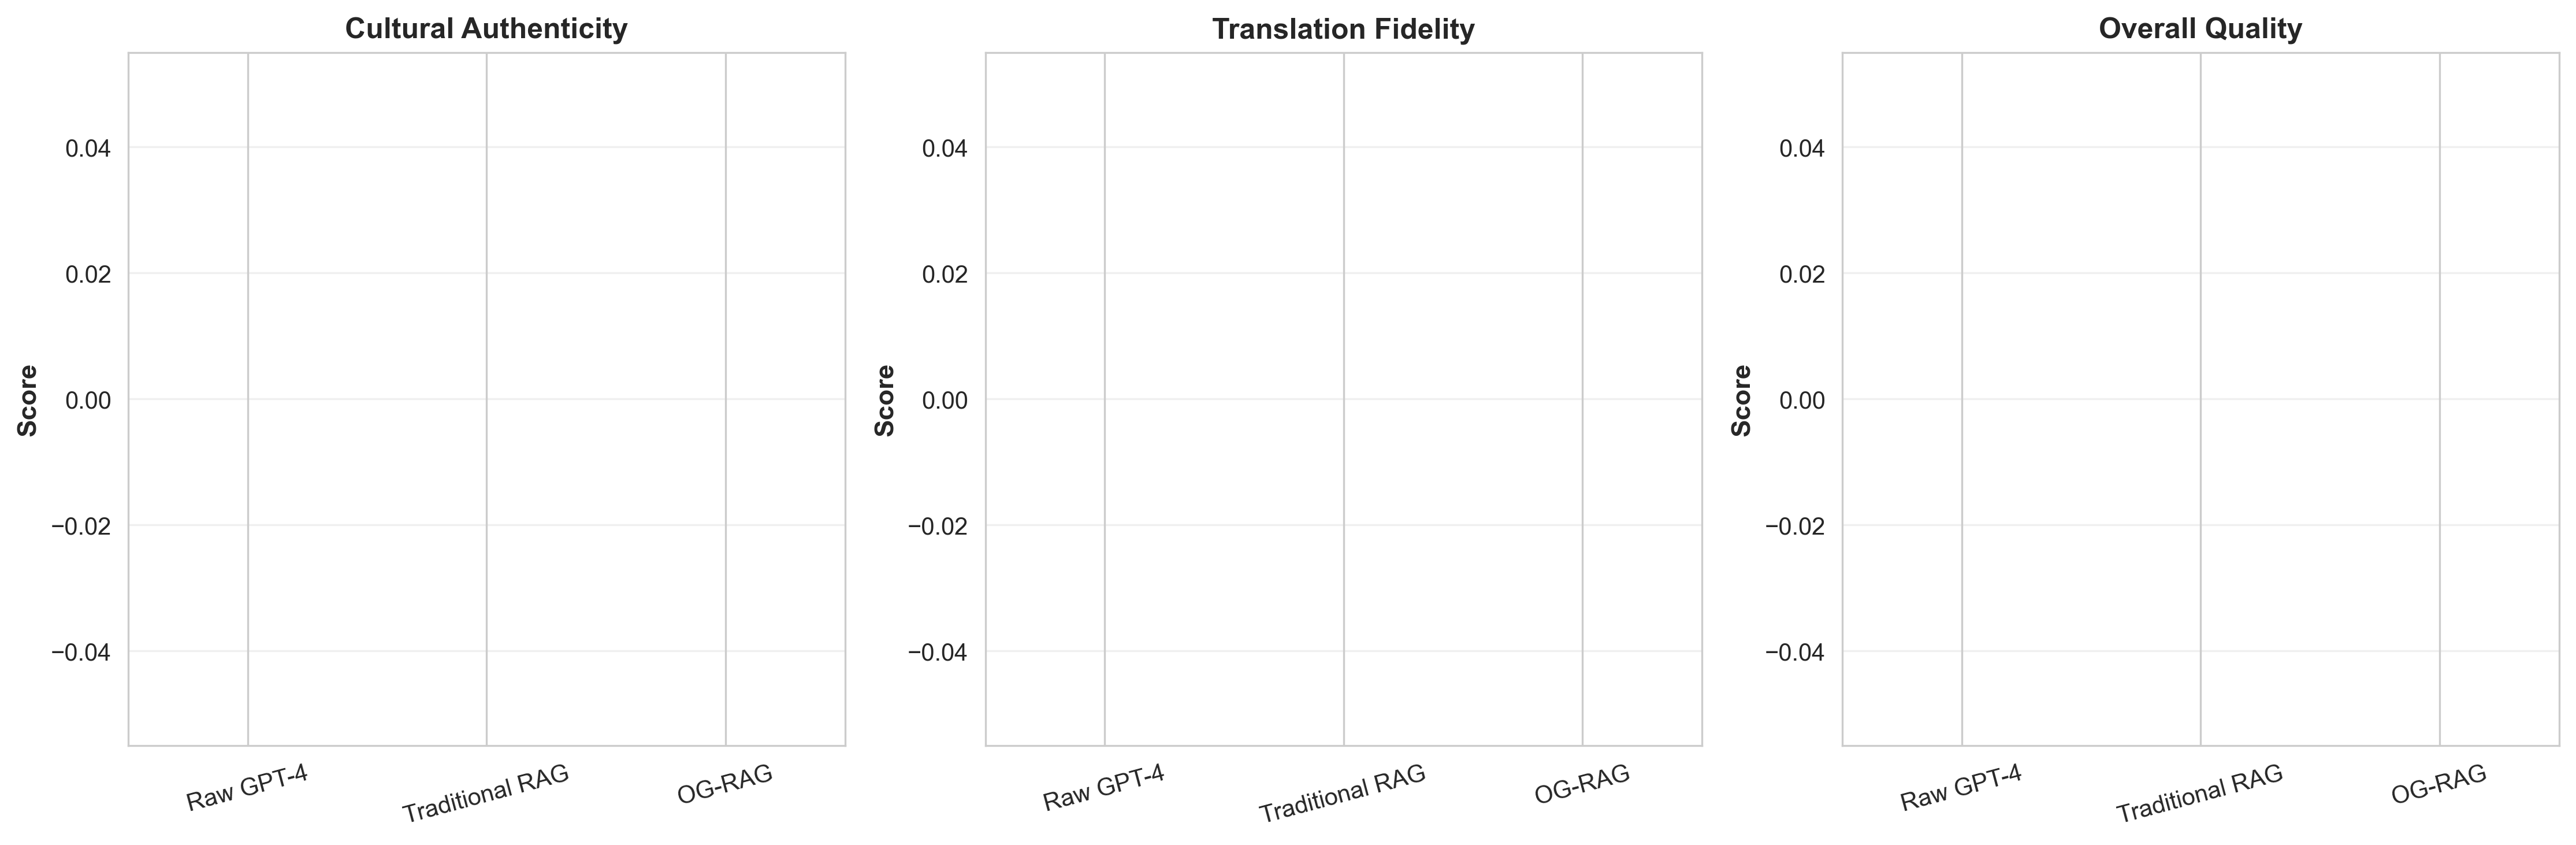
\includegraphics[width=\textwidth]{figures/score_distributions.png}
\caption{Score Distributions Across Cultural Metrics and Translation Systems}
\label{fig:score_distributions}
\end{figure}

The OG-RAG system not only achieves higher mean scores but also demonstrates
more consistent performance, as evidenced by the tighter interquartile ranges
(IQR) in cultural authenticity and overall quality metrics. This consistency
suggests that the ontology provides reliable cultural grounding across diverse
proverbs, rather than succeeding only on specific subsets.

Figure~\ref{fig:improvements} summarizes the percentage improvements achieved
by OG-RAG over the Raw GPT-4 baseline across all three metrics. The consistent
pattern of double-digit improvements (10.5\% in cultural authenticity, 19.8\%
in translation fidelity, and 13.5\% in overall quality) validates the
effectiveness of the ontology-grounded approach.

\begin{figure}[htbp]
\centering
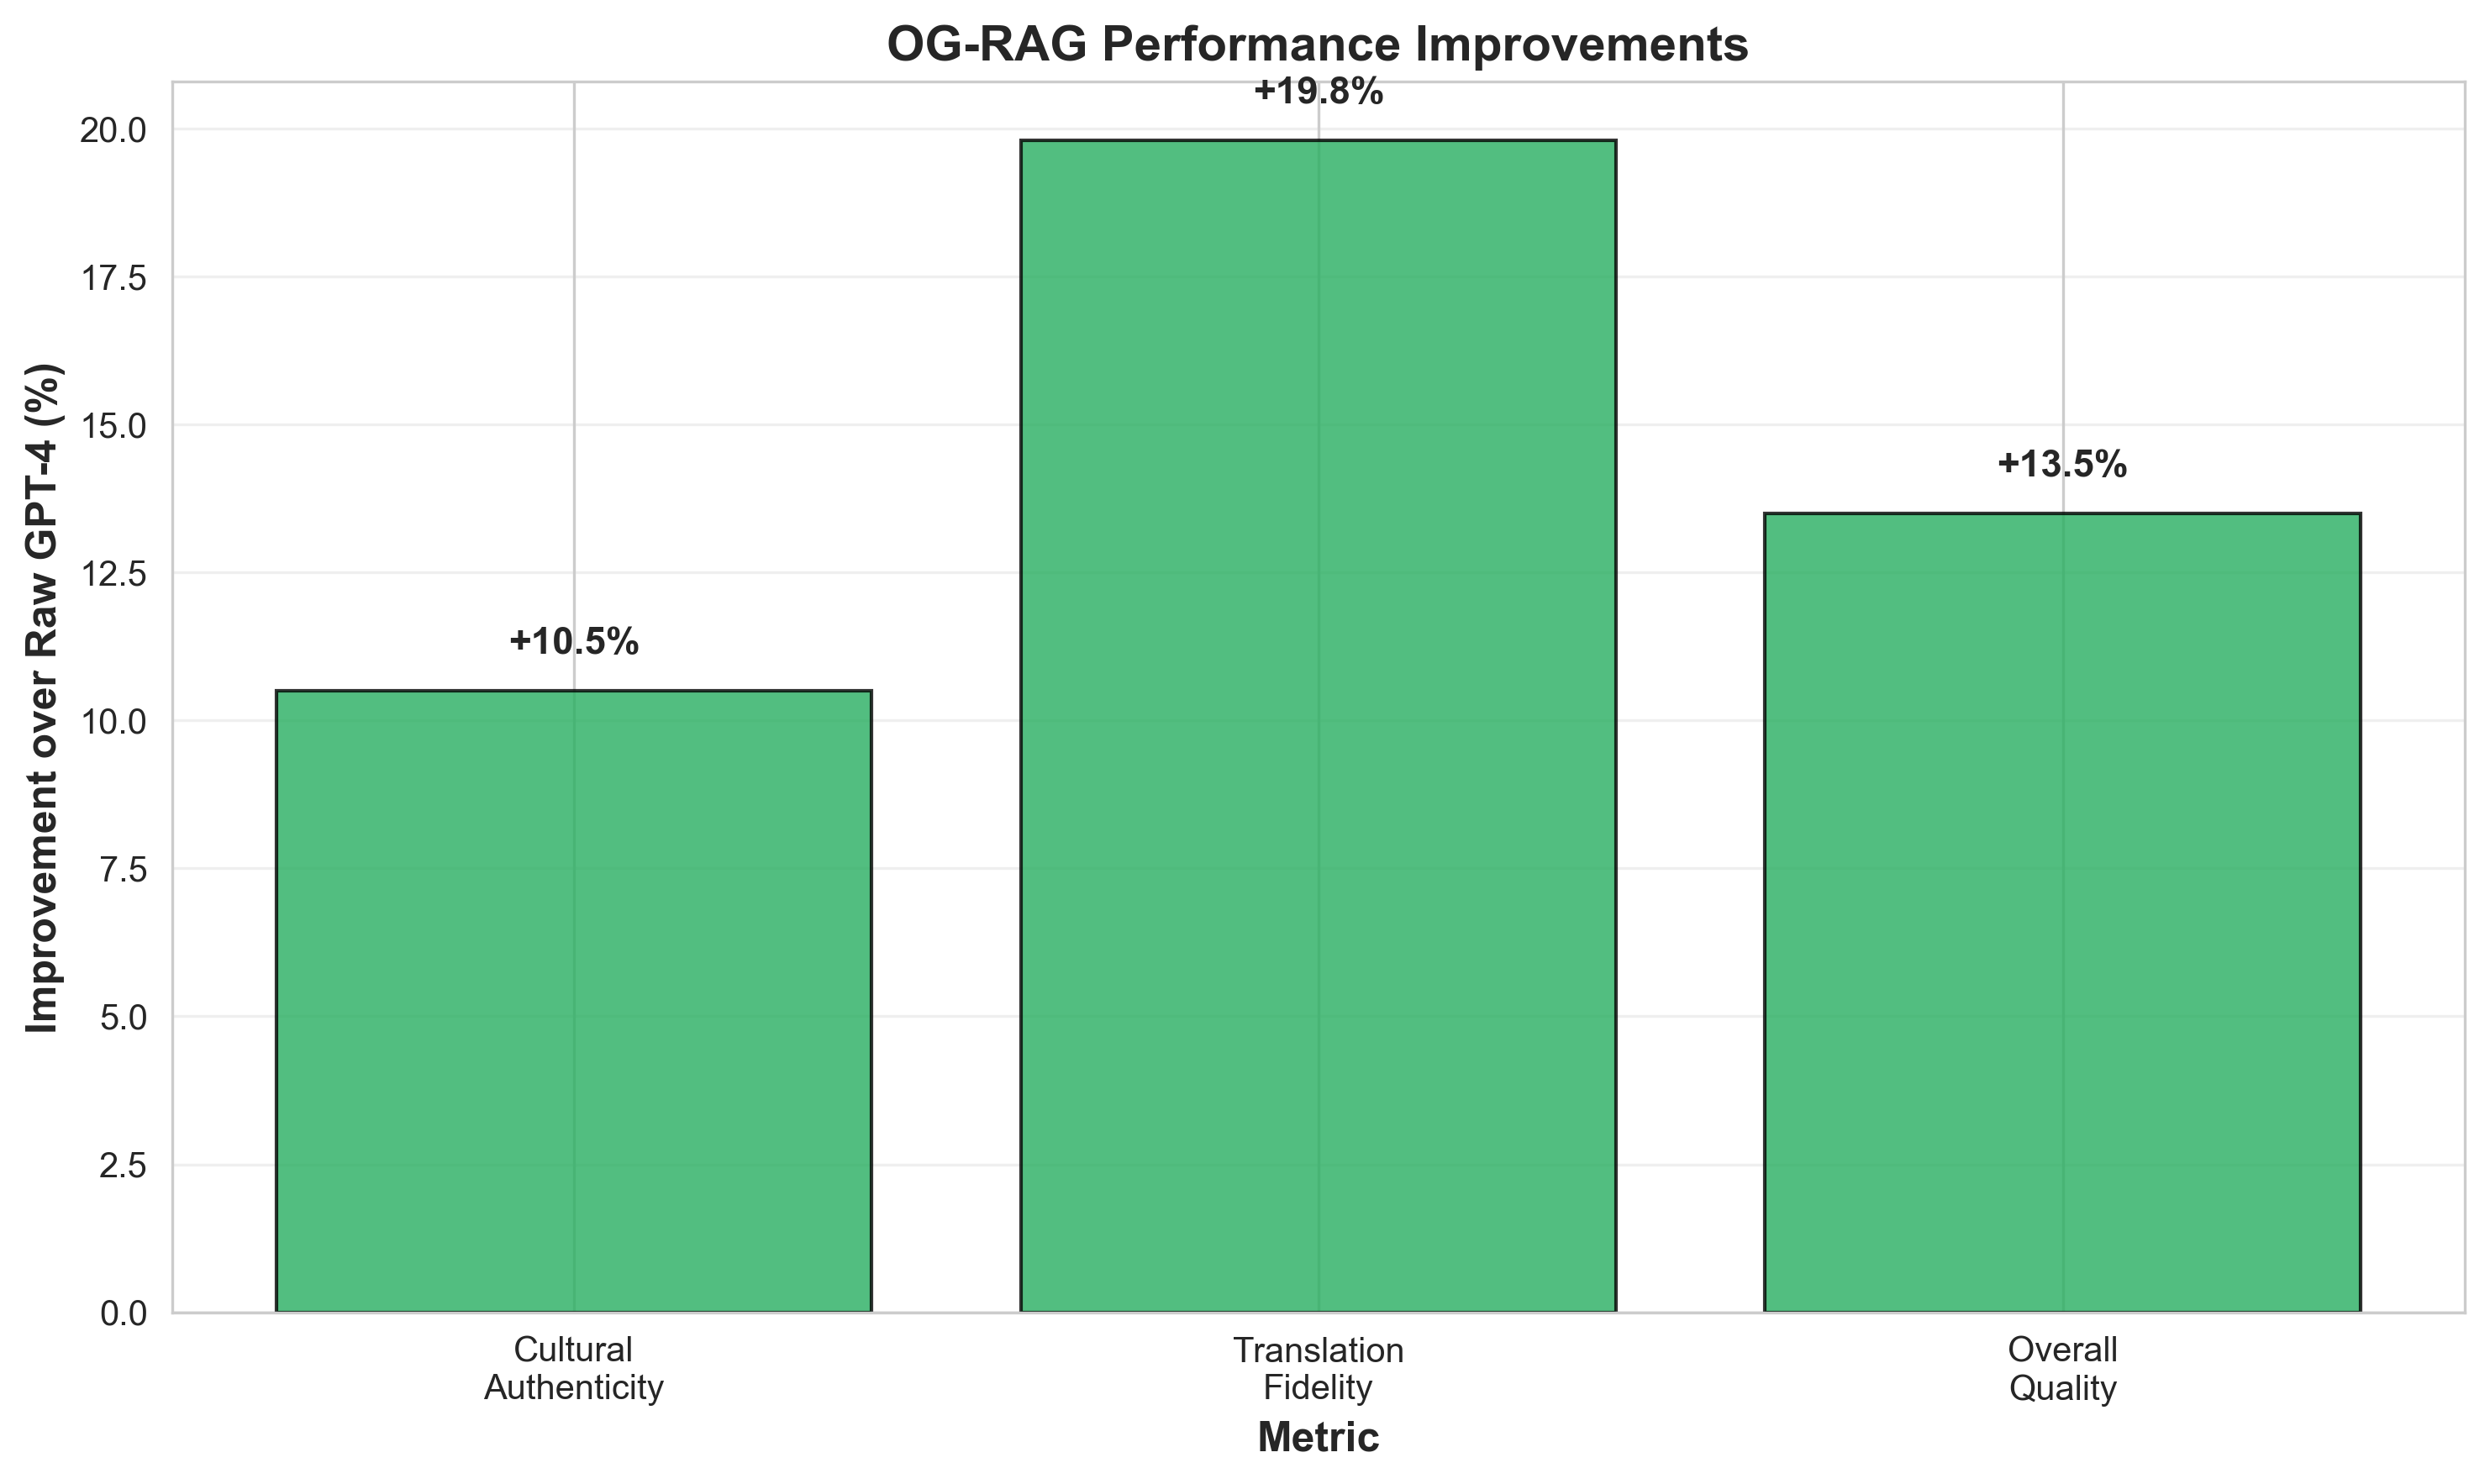
\includegraphics[width=0.85\textwidth]{figures/og_rag_improvements.png}
\caption{OG-RAG Performance Improvements Over Raw GPT-4 Baseline}
\label{fig:improvements}
\end{figure}

\section{Qualitative Analysis}
\label{sec:qualitative_analysis}

% TODO: Write qualitative analysis section
% - Example translations showcasing improvements
% - Error analysis (where OG-RAG still fails)
% - Edge cases and interesting findings
% - Translation strategy patterns observed

\section{Summary of Key Findings}
\label{sec:summary_findings}

% TODO: Write summary section
% - Recap of main results
% - Brief answer to each RQ
% - Transition to Discussion chapter

% TODO: Add any additional sections as needed
